\section{Introduction to network filesystems}

Network file systems allow files on a server to be shared and accessed over the network.
Several different protocols for network file systems have been designed over the years,
with the most well-known being Network File System (NFS) and 
Server Message Block (SMB).
% Common Internet File System (CIFS).
Though history and specifics of those protocols differ considerably, the common design
goal shared by both of them is to be transparent to the applications using them.
That is, applications and libraries should work identically on networked file systems
as they work on local file systems, without requiring any code changes or recompilation.

The NFS protocol originates from Sun Microsystems, where the initial implementation work for the
Unix 4.2 operating system was started in 1984~\cite{NFS}. Its original design goals were
transparent operation with existing programs by maintaining existing Unix file system
semantics, ability to recover from server reboots or crashes, and having reasonable
performance. Since then, extensions to the original protocol have been standardized
in several RFCs, with NFSv3~\cite{NFSv3RFC} in 1995 and NFSv4~\cite{NFSv4RFC},
bringing several improvements in performance, security and feature set~\cite{NFSv4Better}.

The SMB protocol has a more complex history behind it. The protocol was initially designed
and implemented by IBM for the DOS operating system in the 80s
and ran over NetBIOS on the session layer and NBF (NetBIOS frames) on the network and transfer layers~\cite{CifsBook}.
In addition to being a file server, protocol, it is capable of sharing printers and serial ports over the network as well.
Further developments to the protocol were made by Microsoft.
In 1992 parts of the the protocol were specified in an X/Open standard~\cite{XopenSmbSpec}.
In 1996, Microsoft started using the Common Internet File System (CIFS) name for the protocol.

\section{Performance measurements}

As mentioned earlier, good performance was one of the design goals of the NFS protocol.
As a result, various benchmarks for NFS server implementations have been implemented.
One instance of such a benchmark is LADDIS from the 90s~\cite{LADDIS}, designed and named after by
several NFS server vendors at that time (\underline{L}egato Systems, \underline{A}uspex Systems, \underline{D}ata General,
\underline{D}igital Equipment, \underline{I}nterphase and \underline{S}un Microsystems).
It is designed to be a standard benchmark for making performance comparisons across different NFS server implementations
or configurations.
The LADDIS benchmarking software is a synthetic workload generator that talks to the NFS server directly,
without any dependency on the NFS client implementation of the system generating the workload.
The implementation of the benchmark consists of making randomly selected NFS protocol operations
(for instance, creating deleting or reading from a file)
to the server.
The distribution of which operations to perform

\section{Performance differences between protocol revisions}

As was mentioned earlier, good performance was one of the design goals for the NFS protocol,
and since the original protocol implementation additional efforts have been spent improving the performance of the protocol.
Naturally, new versions of the protocol raise the question of how much does an improved protocol revision actually help.
For version 4.1 of the NFS protocol, this has been investigated in the aptly-named article ``Newer Is Sometimes Better: An Evaluation of NFSv4.1''~\cite{NFSv4Better}, which compares NFSv3, NFSv4 and NFSv4.1 performance of the Linux NFS server implementation.
Their test setup was done on a 10GbE network with five client machines and one server machine, running identical enterprise-class hardware.
The NFS server was equipped with fast solid-state disks in RAID-0 to keep the focus of the tests on the protocol level performance.
In addition to comparing performance with multiple clients, the test setup included possibility of adding artificial network latency to the test.

According on the team's analysis on their results, a significant improvement that the version 4.1 of the NFS protocol brings is the \emph{delegation
mechanism} to improve the effectiveness of client-side caching.
Consider an implementation that wishes to do read caching and simultaneously maintain coherency in case of other clients
concurrently writing to the same file.
In the stateless NFSv3 protocol, the client doing the reads must periodically ask the server for the last-modification timestamp of the file in order to notice other clients writing to the file.
The read delegation feature of NFSv4.1 allows a better way of managing caching.
The server now maintains state for opened files, so a lone client reading files can proceed with full caching,
and in case some other client starts writing concurrently, the server will notify the client and recall the delegation.

For concrete numbers on the benefits of delegations, a microbenchmark of repeatedly reading (10 times per file) 10 000 small files performs X times faster.
On the protocol level, NFSv3 performed 20 times the amount of NFS requests compared to NFSv4.1 with delegations enabled.
% XXX this microbenchmark is different from the one in the graph below.

However, the delegations feature is not an universal improvement.
The need for OPEN and CLOSE requests to maintain state of open files on the server can significantly increase the amount of protocol requests made by NFSv4.1 compared to NFSv3.
For instance, the file server workload of the Filebench benchmark caused an increase of 56\% in the number of protocol requests made by NFSv4.1 over NFSv3.
This translated into a 8--18\% of slowdown.
% The biggest difference was in the zero-delay network, where V4.1p was 15% slower

\begin{figure}[h]
\centering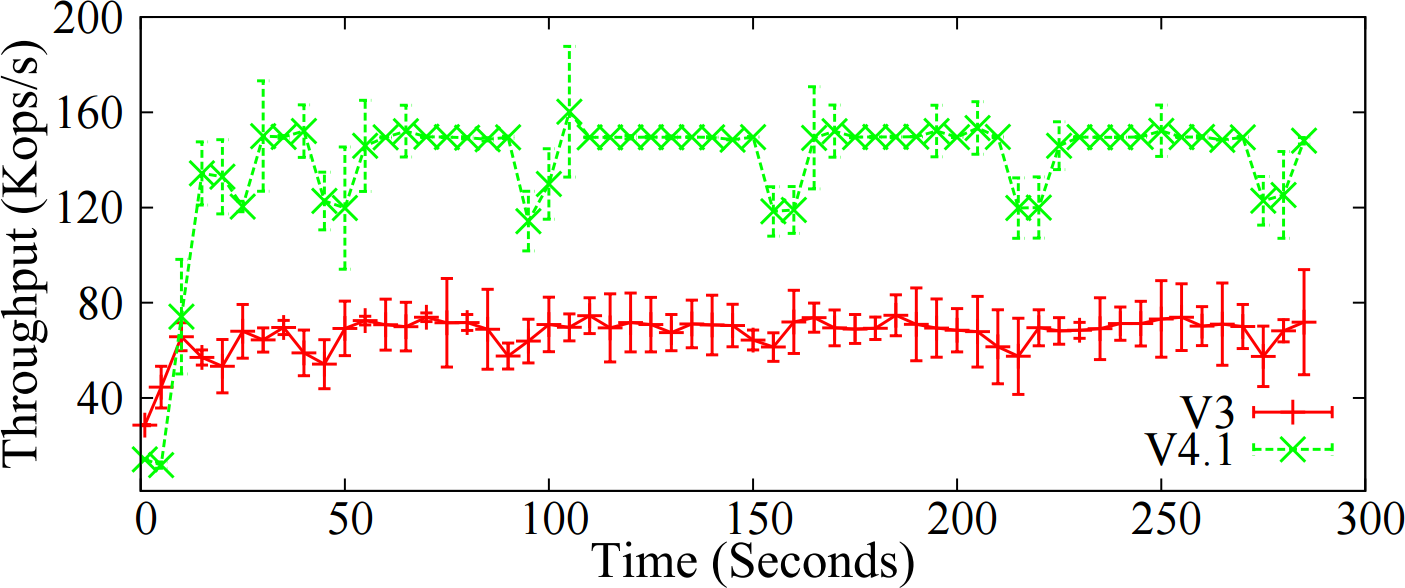
\includegraphics[width=0.8\textwidth]{images/nfsv41better-reading-small-files.png}
\caption{Figure 6 from ``Newer Is Sometimes Better: An Evaluation of NFSv4.1''~\cite{NFSv4Better}.}
% Section 4.1 Read Small Files
\end{figure}

\section{Analysis of a production file server}

Another approach of analysing network file systems is to look at how the actual users of such systems are using it.
One such example comes from ``Measurement and Analysis of Large-scale Network File System Workloads''~\cite{NetApp} done by NetApp,
a company developing network storage products.
The study was done on the corporate's own internal 22 TB file servers by collecting live packet captures of CIFS protocol traffic.
Compared to other ways of collecting data on file server usage, such as analysing static file system snapshots of the file server,
the use of network traffic as a data source allows analysis of changes to the file system over time.
Since user authentication in the test environment was done by a separate Kerberos protocol,
only IP addresses were used to correlate CIFS sessions to actual unique users of the system.
